% 原书 p.70–p.75（PDF p.78–p.83）
\section{勒让德子流形（Legendrian Submanifolds）}

\begin{keytakeaways}
\begin{itemize}
  \item 几何图像：勒让德子流形是切触流形中「切于切触超平面」且维数最大的子流形
        （$\dim L=(\dim M-1)/2$）；在 $\R^3$ 中它们是勒让德曲线，可由其
        $xz$-平面上的前沿投影恢复。
  \item 数学工具：可积子平面场的维数上界（由 $\dd\alpha|_\xi$ 非退化得到）、
        $1$-jet 丛 $J^1Q=T^*Q\times\R$ 中的生成函数图 $\Gamma_f$、单位余法丛
        $\Lambda_N$、$C^0$-逼近（命题 3.4.1）。
  \item 本节结论：$\Gamma_f$ 与 $\Lambda_N$ 是勒让德子流形的两大来源；勒让德纽结
        的尖点、交叉与 Reeb 弦是研究其不变量的几何要素；Arnold 弦猜想是
        Weinstein 猜想的勒让德对应物。
\end{itemize}
\end{keytakeaways}

% >>> p078
回忆 §1.6 中引入拉格朗日子流形的动机：辛形式 $\omega$ 在整个流形的切丛上
非退化，但限制到子流形的切丛上可能退化。类似地，在切触流形 $(M,\xi)$ 上，
切触结构 $\xi$ 在 $M$ 上完全不可积，并不意味着它的子平面场不可积。例如，
$\xi$ 的任何（光滑）一维子平面场——它无非是 $M$ 上的一个光滑向量场——总是
可积的。

一般地，设 $\eta\subset\xi$ 是 $\xi$ 的可积子平面场。回忆 $\eta$ 可积当且
仅当对任意 $X,Y\in\eta$，其泊松括号满足 $[X,Y]\in\eta$。同时，对任意
$1$-形式 $\alpha$，有下述等式：
\[
  \dd\alpha(X,Y)=X(\alpha(Y))-Y(\alpha(X))-\alpha([X,Y]).
\]
若取切触 $1$-形式 $\alpha$ 使 $\xi=\ker\alpha$，则对任意 $X,Y\in\eta$
（特别地，$X,Y\in\xi=\ker\alpha$）都有 $\dd\alpha(X,Y)=0$。换言之，
$\dd\alpha|_\eta\equiv0$。于是，由 §3.1 中的观察 (iv)——$\dd\alpha|_\xi$
非退化——$\eta$ 的可积性蕴含其维数不超过 $(\dim M-1)/2$。

下一个定义是定义 1.6.1 的类比物：它给出切触结构中能承载可积子平面场的、
维数最大且整体定义的子流形。

\begin{wdefn}{3.4.1}
设 $(M,\xi)$ 是切触流形。\textbf{勒让德子流形}（Legendrian submanifold）
$L\subset M$ 是指满足下述条件的子流形：(i) $TL\subset\xi$；
(ii) $\dim L=(\dim M-1)/2$。
\end{wdefn}

\begin{wrem}{3.4.1}
给定勒让德子流形 $L\subset(M,\xi)$，切触结构 $\xi$ 的任何切触 $1$-形式
$\alpha$ 在 $TL$ 上为零。与拉格朗日情形中辛结构「看不见」子流形的道理类似，
任何切触 $1$-形式也都「看不见」勒让德子流形（它是切触流形中最重要的一族
子流形）。
\end{wrem}

\begin{wrem}{3.4.2}
通有地，两个勒让德子流形不相交。这纯粹是维数上的原因。事实上，对勒让德
子流形 $L,L'\subset(M^{2n+1},\xi)$，若它们横截相交，则
\[
  \operatorname{codim}(L\cap L')
  =\operatorname{codim}L+\operatorname{codim}L'=2n+2,
\]
% >>> p079
这与 $M^{2n+1}$ 的整体维数矛盾。
\end{wrem}

下面列举勒让德子流形的若干重要例子。

\begin{wexam}{3.4.1}
回忆 $T^*Q$ 上一族拉格朗日子流形可由闭 $1$-形式的图构造（见例 1.6.3），
特别地可由恰当 $1$-形式 $\dd f$（$f:Q\to\R$）的图构造。循此思路，可以在
\textbf{$1$-jet 丛} $J^1Q:=T^*Q\times\R$ 中构造勒让德子流形。空间
$J^1Q$ 可看作余切丛 $(T^*Q,\dd\lambda_{\mathrm{can}})$ 的切触化的某种版本
（参看例 3.2.2）。这里我们取切触 $1$-形式为
$\alpha:=\lambda_{\mathrm{can}}+\dd r$，其中 $r$ 是 $\R$ 分量的参数。

给定任意可微函数 $f:Q\to\R$，考虑如下子流形：
\[
  \Gamma_f:=\bigl\{(q,\dd f(q),-f(q))\ \big|\ q\in Q\bigr\}\subset J^1Q .
\]
它是勒让德子流形，因为
$i^*\alpha=i^*(\lambda_{\mathrm{can}}+\dd r)=\dd f-\dd f=0$，其中
$i:\Gamma_f\to J^1Q$ 是嵌入，且
$\dim\Gamma_f=\dim Q=(\dim J^1Q-1)/2$。\hfill$//$
\end{wexam}

\begin{wrem}{3.4.3}
作为 Weinstein 邻域定理（见定理 4.3.3）的类比：切触流形 $(M,\xi)$ 中任何
紧勒让德子流形 $L$ 都有邻域，可在切触意义下等同于 $J^1L$ 中零截面的邻域
（见练习 4.3.1）。这里 $J^1L$ 中的零截面是指子流形
$\{(x,0,0)\in T^*L\times\R\mid x\in L\}$。
\end{wrem}

\begin{wexam}{3.4.2}
对例 3.2.1 中考虑的欧氏空间
$(\R^3,\xi_{\mathrm{std}}=\ker(\dd z-y\,\dd x))$，勒让德子流形是
一维的（即曲线），于是可把任意勒让德子流形 $L$ 参数化如下：
\[
  L=\bigl\{\gamma(t):=(x(t),y(t),z(t))\in\R^3\ \big|\ t\in I\bigr\},
\]
其中 $I\subset\R$ 是某区间。由于此曲线以 $[0,1]$ 为参数（有序），沿 $L$
移动时便带有相应的定向。$L$ 的切空间由下式给出：
\[
  T_{\gamma(t)}L
  =x'(t)\frac{\partial}{\partial x}+y'(t)\frac{\partial}{\partial y}
  +z'(t)\frac{\partial}{\partial z}.
\]
在标准切触 $1$-形式 $\dd z-y\,\dd x$ 下，勒让德条件
$T_{\gamma(t)}L\subset(\xi_{\mathrm{std}})_{\gamma(t)}$ 等价于
$z'(t)-y(t)x'(t)=0$。若 $x'(t)\neq0$，这等价于
\begin{equation}\tag{3.26}
  y(t)=\frac{z'(t)}{x'(t)} .
\end{equation}
换言之，对那些满足 $x'(t)\neq0$ 的 $t$，坐标 $y(t)$ 可由 $z'(t)$ 与
$x'(t)$ 还原出来。

实现这一点的系统办法是考虑 $L$ 到 $xz$-平面的投影。(3.26) 的右端
$z'(t)/x'(t)$ 恰是点 $(x(t),y(t),z(t))$ 处沿勒让德子流形 $L$ 的斜率。
因此，坐标 $y(t)$ 可以直接从投影的图读出
% >>> p080
（该投影通常称为 $L$ 的\textbf{前沿投影}（front projection））。图 3.11
说明了如何由 $L$ 的前沿投影上的点恢复 $\R^3$ 中 $L$ 上的点。\hfill$//$
\end{wexam}

\begin{figure}[htbp]
  \centering
  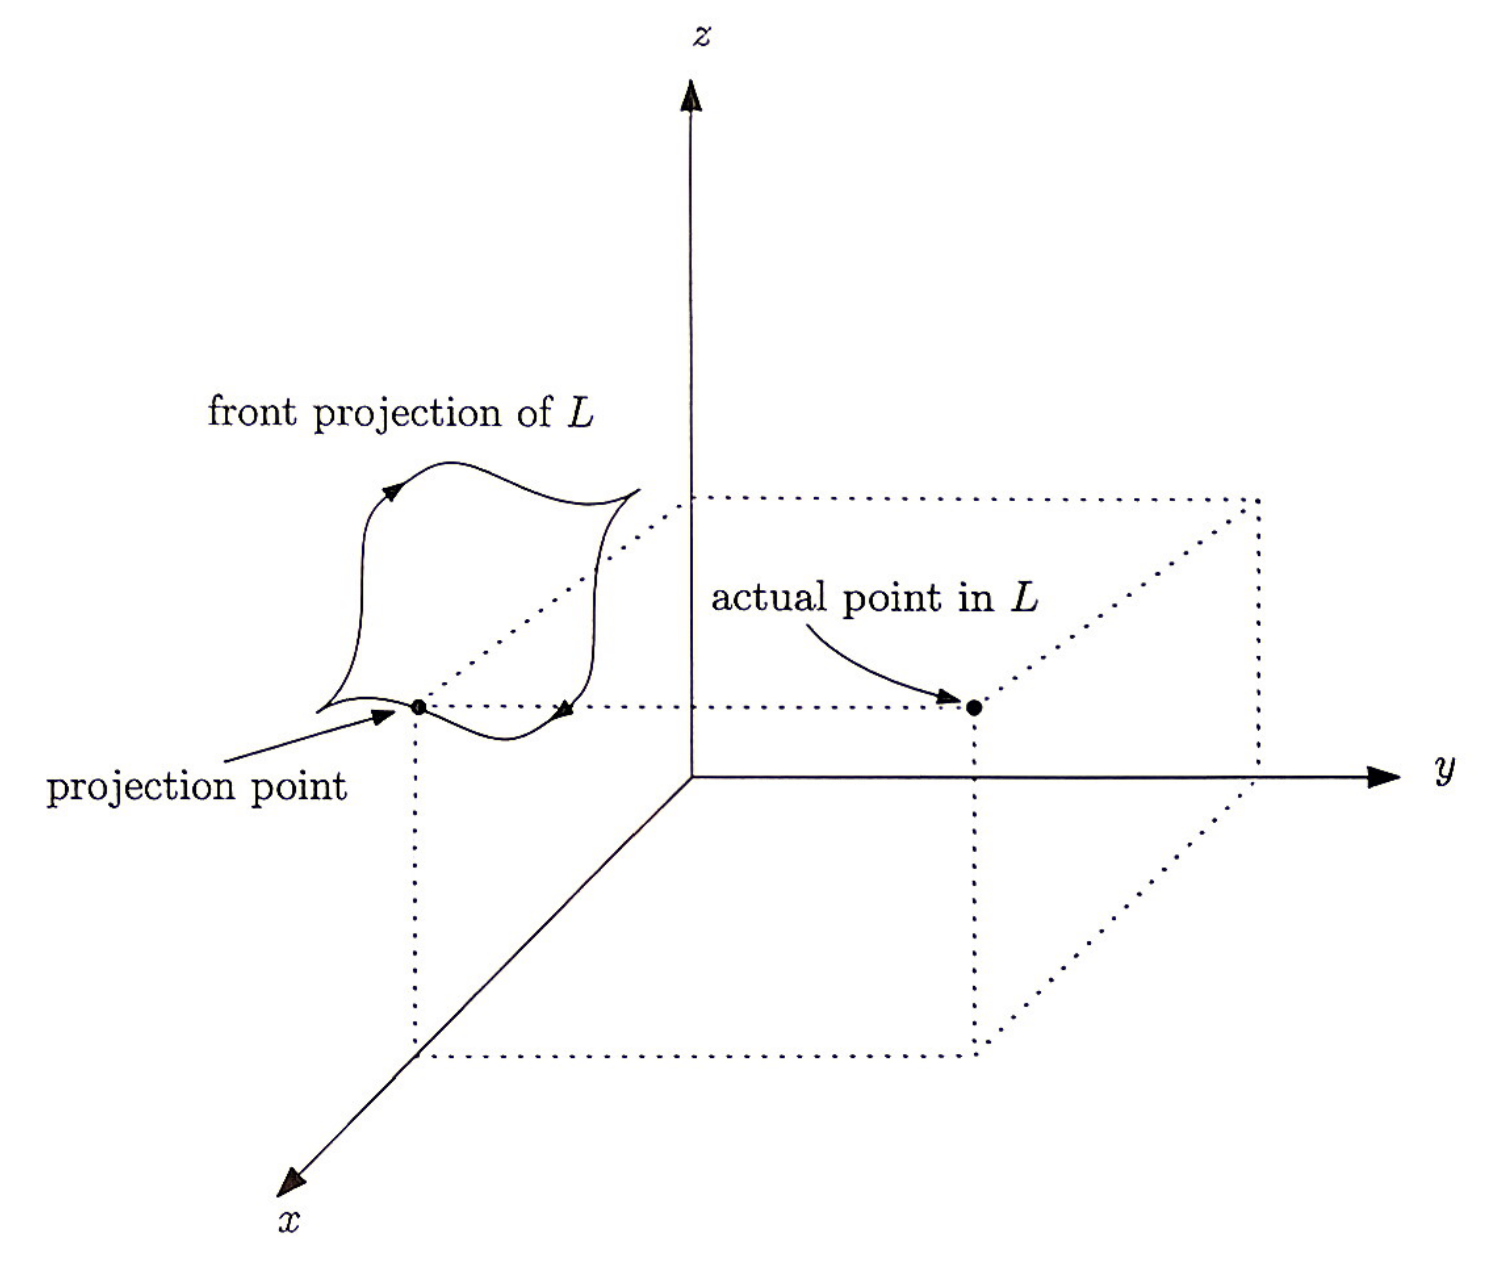
\includegraphics[width=0.56\linewidth]{figures/fig_p080_1.png}
  \caption*{图 3.11\quad $L$ 在 $xz$-平面上的前沿投影
  （原书 p.72, Figure 3.11）}
\end{figure}

\begin{wrem}{3.4.4}
设 $L$ 紧，则 $L$ 的 $y$-坐标总是有限的（因此在前沿投影中永远不会看到竖直
切线）。一般地，由方程 $z'(t)-y(t)x'(t)=0$ 可得四种情形。
\begin{enumerate}[label=(\roman*)]
  \item 当 $z'(t)=0$ 而 $x'(t)\neq0$ 时，$y(t)=0$。这对应于前沿投影中所有
        具有水平切线的点。
  \item 当 $z'(t)=0$ 且 $x'(t)=0$ 时，这意味着前沿投影曲线在此点终止。由于
        $L$ 是连续曲线，相应的 $y$-坐标将由附近点的信息确定。
  \item 当 $z'(t)\neq0$ 而 $x'(t)=0$ 时，这是不可能的。
  \item 当 $z'(t)\neq0$ 且 $x'(t)\neq0$ 时，这是正则点，$y$ 可由方程
        (3.26) 算出。
\end{enumerate}
\end{wrem}

\begin{wexam}{3.4.3}
$\R^3$ 中的勒让德子流形可以与纽结理论相结合。回忆 $\R^3$ 中的\textbf{纽结}
（knot）是指光滑嵌入 $S^1\hookrightarrow\R^3$ 的像。\textbf{勒让德纽结}
（Legendrian knot）是指这样的像同时是
$(\R^3,\xi_{\mathrm{std}}=\ker(\dd z-y\,\dd x))$ 中的勒让德子流形
（已在例 3.4.2 中讨论）。对 $\R^3$ 中任意勒让德纽结 $\gamma$，可考虑其在
$xz$-平面中的前沿投影 $\gamma_F$。这里有两个显著的几何要素。
% >>> p081
其一是 $\gamma_F$ 中\textbf{尖点}（cusp）的存在（见图 3.12 的第一幅图）。
它对应于注 3.4.4 中的第 (iii) 项：前沿投影曲线在此终止，随后 $x'(t)$ 改变
符号。其二是 $\gamma_F$ 中的\textbf{交叉点}（crossing）（见图 3.12 的第二
幅图）。由 (3.26)，这对应于 $L$ 中两个具有相同 $x$-坐标与 $z$-坐标、但
$y$-坐标不同的点（一个 $y>0$，另一个 $y<0$）。

\begin{figure}[htbp]
  \centering
  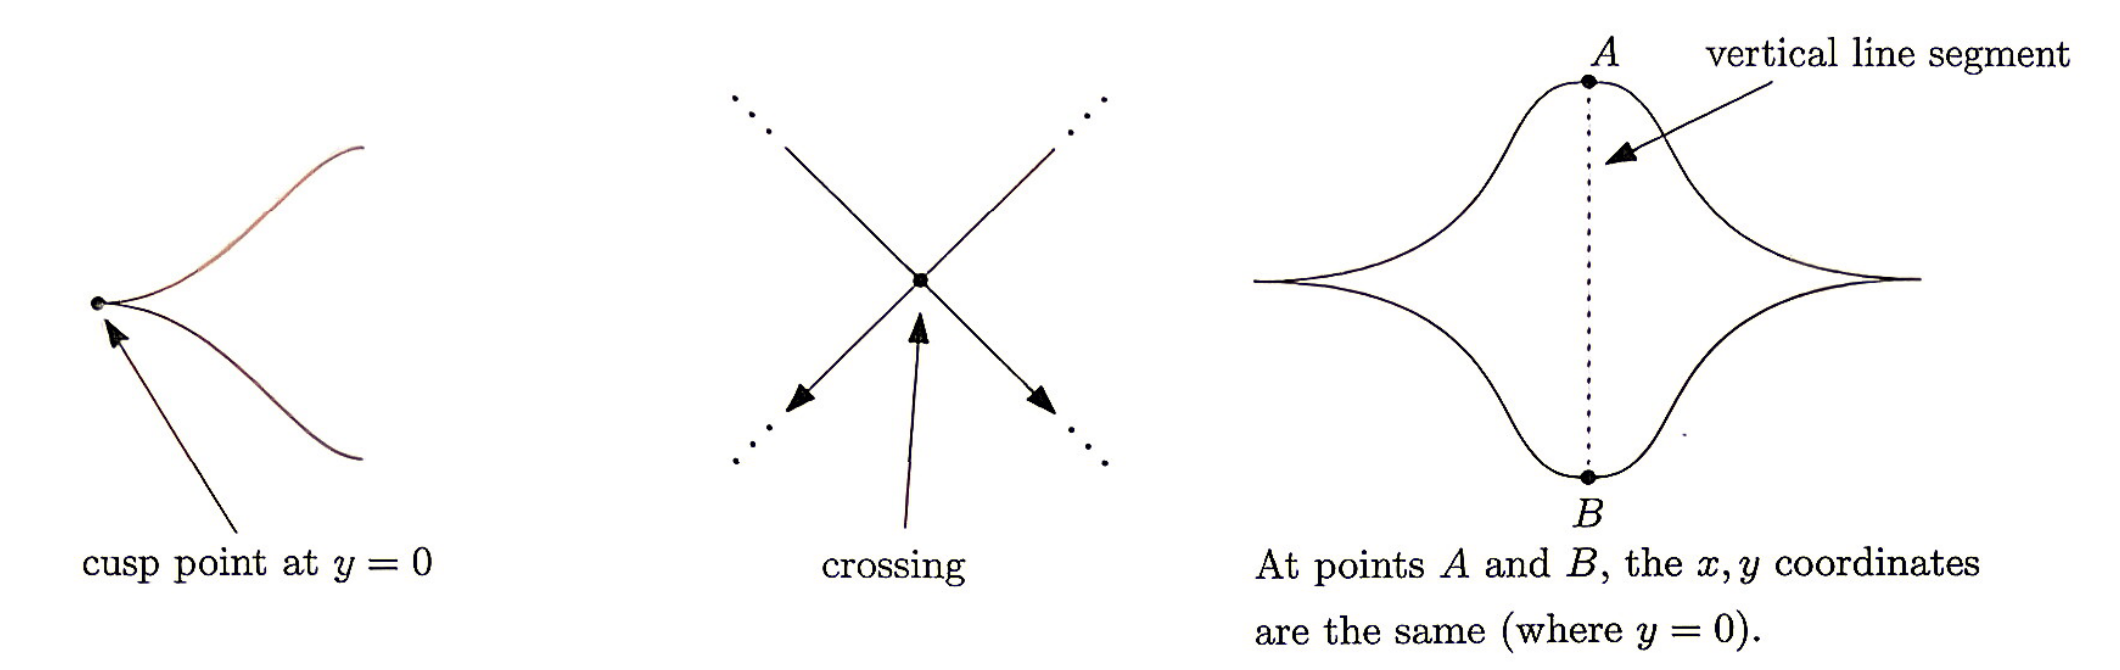
\includegraphics[width=0.85\linewidth]{figures/fig_p081_1.png}
  \caption*{图 3.12\quad 尖点与竖直截段
  （原书 p.73, Figure 3.12）}
\end{figure}

% [Tutor Note: 原文疑误——正文称尖点「对应于注 3.4.4 中的第 (iii) 项」，但
% 注 3.4.4 的第 (iii) 项是「$z'\neq0$ 而 $x'=0$，不可能」，真正描述前沿投影
% 曲线终止的是第 (ii) 项（$z'=x'=0$）。$C^0$ 意义上尖点的参数化恰是 $x'$ 变号
% 而 $x'=z'=0$ 的退化点。已记入 review_ch03.md。]

勒让德纽结理论内容非常丰富。作为一个初等的例子，（勒让德）纽结 $L$ 的若干
经典不变量（例如记为 $\mathrm{tb}(L)$ 的 Thurston–Bennequin 不变量，或
记为 $r(L)$ 的旋转数）都可由上述几何要素计算出来。更多细节见 [125] 的 §3.5。

最后我们要强调另一对有趣的点——它们具有相同的 $x$-坐标与 $y$-坐标，但
$z$-坐标不同（见图 3.12 的第三幅图）。注意在
$(\R^3,\xi_{\mathrm{std}}=\ker(\dd z-y\,\dd x))$ 中，Reeb 向量场为
$\partial/\partial z$。因此这对点位于同一条 Reeb 流线上，而把一点带到另一点
的那段流线称为 \textbf{Reeb 弦}（Reeb chord）。与 Weinstein 猜想（见猜想
3.1.1）类似，给定闭切触流形 $(M,\xi=\ker\alpha)$ 中的勒让德子流形 $L$，
寻找 Reeb 弦同样是困难问题——相关猜想称为 \textbf{（强）Arnold 弦猜想}
（(strong) Arnold chord conjecture，参看 [14, 129, 130, 162, 133]）。更精确
的陈述见猜想 5.3.4。\hfill$//$
\end{wexam}

% [Tutor Note: 术语依据——Reeb chord 通行译名为「Reeb 弦」，与「Reeb 轨道」
% 并列为 Reeb 动力学的两大对象：闭轨道是闭 Reeb 流的周期解，而 Reeb 弦是
% 连接两个给定点（这里是勒让德子流形上的两点）的流线段。Arnold 弦猜想断言
% 紧切触流形中任何勒让德子流形都存在 Reeb 弦；它与 Weinstein 猜想通过
% 「在辛化中把闭轨道切成两条弦」相联系。]

由于方程 (3.26)，在
$(\R^3,\xi_{\mathrm{std}}=\ker(\dd z-y\,\dd x))$ 中构造勒让德子流形，可以
系统地由 $xz$-平面中的「前沿投影型」曲线得到。事实上，这一方法蕴含下述有趣
的命题，它与 $C^0$-逼近有关；这也说明在
$(\R^3,\xi_{\mathrm{std}}=\ker(\dd z-y\,\dd x))$ 中确实存在大量的勒让德
子流形。

\begin{wprop}{3.4.1}（[92] 中定理 3.3.1）
在切触流形
$(\R^3,\xi_{\mathrm{std}}=\ker(\dd z-y\,\dd x))$ 中，任何光滑道路
$\gamma=\{(x(t),y(t),z(t))\mid t\in[0,1]\}$ 都可在 $C^0$-拓扑下被勒让德
道路逼近。确切地说，对任意 $\varepsilon>0$，存在勒让德道路
$L=\{(a(t),b(t),c(t))\mid t\in[0,1]\}$，使得
\[
  \max_{t\in[0,1]}|\gamma(t)-L(t)|\le\varepsilon,
\]
其中 $|\cdot|$ 表示 $\R^3$ 中的标准范数。
\end{wprop}

% >>> p082
\begin{wproof}
这里给出证明梗概。记光滑道路 $\gamma$ 的前沿投影为 $\gamma_F$。可用
$xz$-平面中的前沿投影型曲线 $\eta$ 在 $C^0$ 意义下逼近 $\gamma_F$，并让
$\eta$ 含有足够多的尖点，使得这条「锯齿状」$\eta$ 沿线的斜率始终与 $\gamma$
的 $y(t)$ 值在 $C^0$ 意义下接近。于是由上述讨论，从 $\eta$ 恢复出的勒让德
曲线 $L\subset\R^3$ 就在 $C^0$ 意义下接近初始给定的 $\gamma$。示意图见
图 3.13。
\end{wproof}

\begin{figure}[htbp]
  \centering
  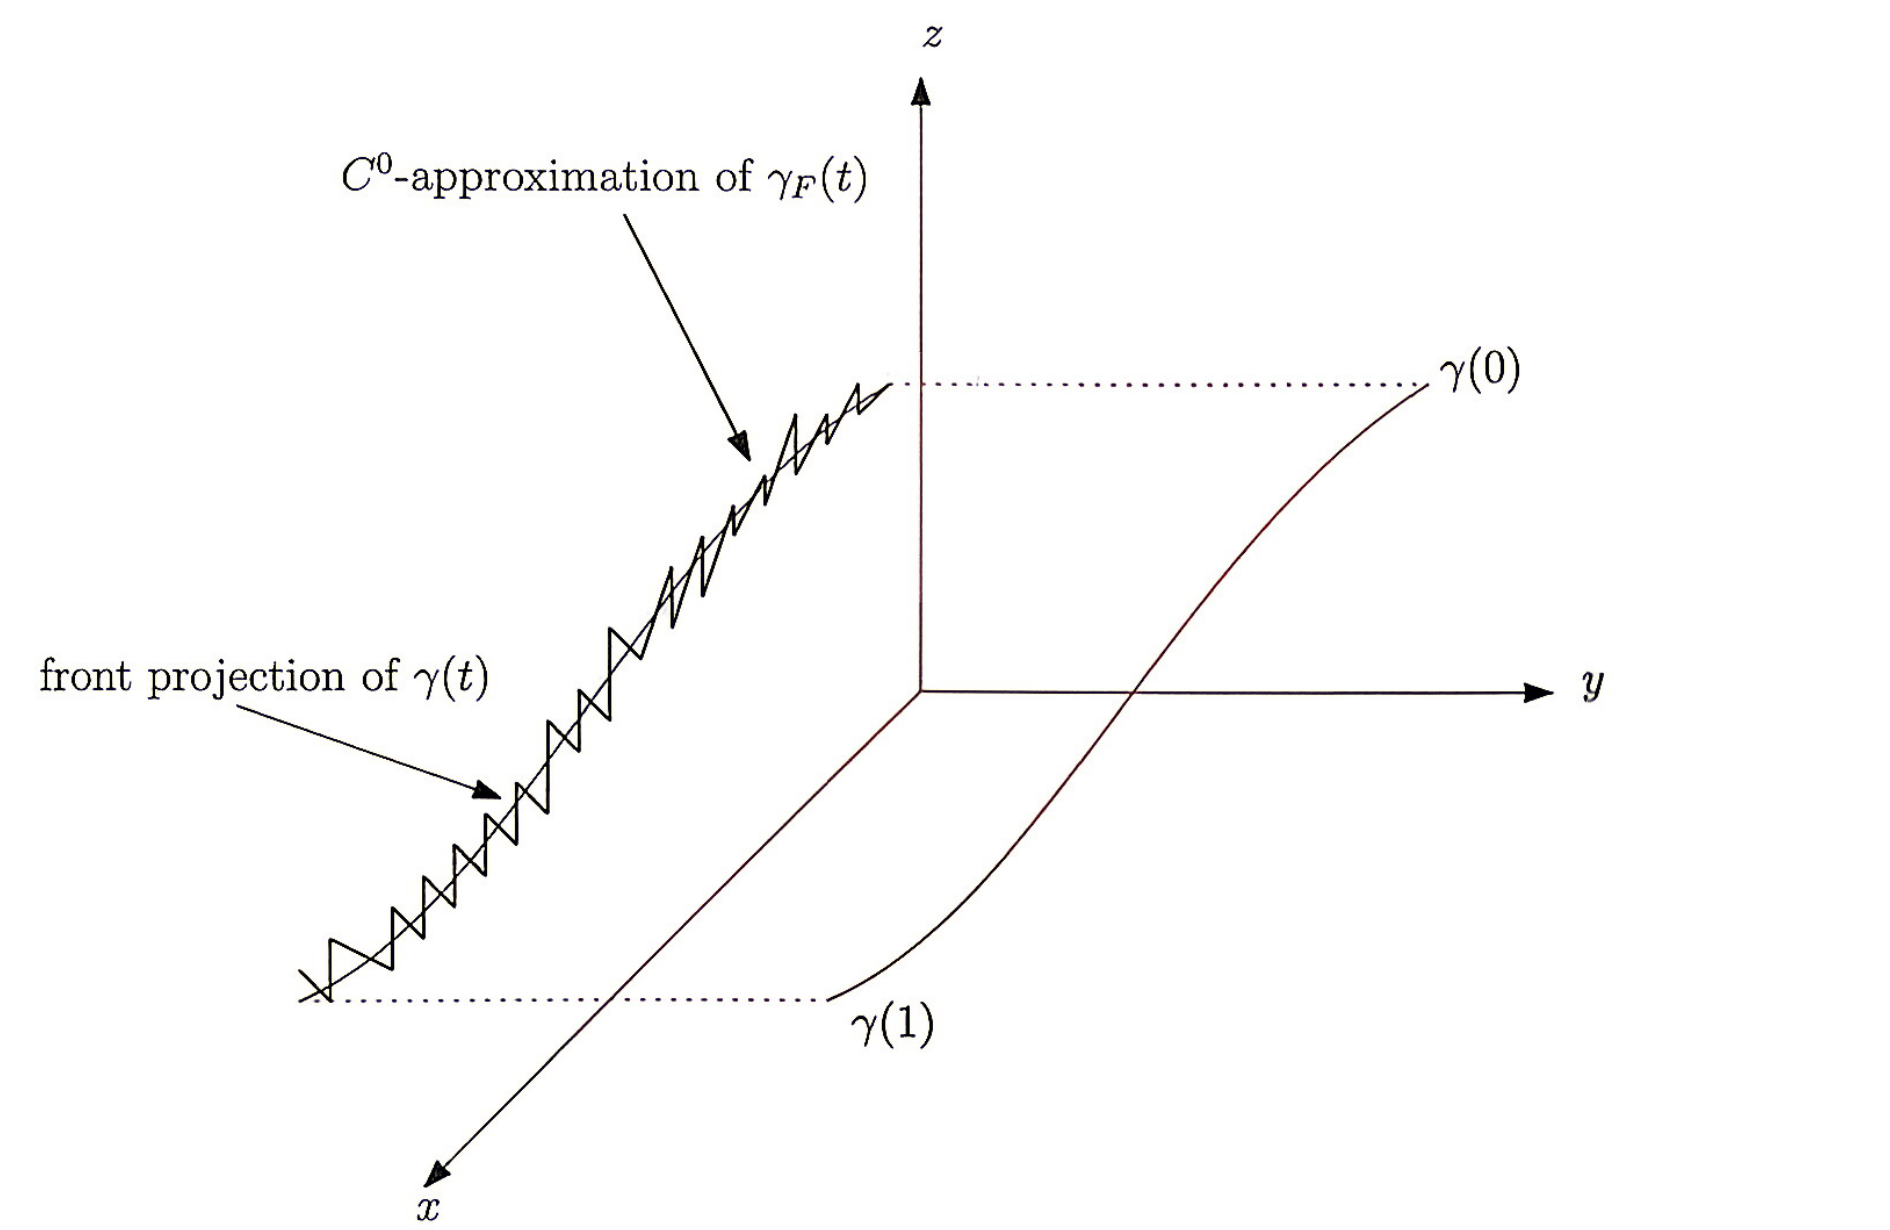
\includegraphics[width=0.58\linewidth]{figures/fig_p082_1.png}
  \caption*{图 3.13\quad 一条 $C^0$-逼近 $\gamma_F(t)$ 的锯齿曲线
  （原书 p.74, Figure 3.13）}
\end{figure}

% [Tutor Note: 含糊点拨——证明梗概中的关键是把「斜率」$y(t)$ 编码到前沿投影
% 的切线斜率中：由 (3.26)，前沿投影在每点的斜率就是该点的 $y$ 值。所谓
% 「锯齿状」曲线，是指在每个小段上以几乎恒定的斜率上升、再以尖点折返，从而
% 用大量短线段逐点拟合连续函数 $y(t)$；尖点处 $x'$ 变号保证了 $x$ 单调性的
% 局部破坏是可控的。$C^0$-逼近不控制导数，故这种「用尖点换取斜率」的技巧
% 可行，这正是命题能成立的原因。]

\begin{wexam}{3.4.4}（单位余法丛）
回忆例 3.2.4 中引入的切触流形
$(S^*_gQ,\lambda_{\mathrm{can}}|_{S^*_gQ})$，即 $(Q,g)$ 的单位余球面丛
（见 (3.12)）。设 $\dim Q=n$，$N\subset Q$ 是维数为 $k\le n-1$ 的子流形。
定义 $N$ 的\textbf{单位余法丛}（unit conormal bundle）为
\begin{equation}\tag{3.27}
  \Lambda_N:=\bigl\{(q,p)\in S^*_gQ\ \big|\ q\in N,\ p|_{TN}=0\bigr\}
  \subset S^*_gQ .
\end{equation}
$\Lambda_N$ 的维数为
\[
  \dim\Lambda_N=k+(n-k-1)=n-1=(\dim S^*_gQ-1)/2,
\]
% >>> p083
其中 $k$ 来自子流形 $N$ 的维数，$n-k-1$ 来自 (3.27) 中的限制条件
$p|_{TN}=0$。事实上，$\Lambda_N$ 是勒让德子流形，这由下述练习确认。

\begin{wexer}{3.4.1}
设 $\Lambda_N$ 是 (3.27) 中定义的子流形。证明 $\Lambda_N$ 是
$(S^*_gQ,\lambda_{\mathrm{can}}|_{S^*_gQ})$ 的勒让德子流形。
\end{wexer}

还有另一种方式引入 $\Lambda_N$。考虑
\begin{equation}\tag{3.28}
  \overline{\Lambda}_N
  :=\bigl\{(q,p)\in T^*Q\ \big|\ q\in N,\ p|_{TN}=0\bigr\}\subset T^*Q .
\end{equation}
容易验证 $\overline{\Lambda}_N$ 是 $(T^*Q,\dd\lambda_{\mathrm{can}})$ 的
拉格朗日子流形。于是 $\Lambda_N=\overline{\Lambda}_N\cap S^*_gQ$。来看
$\Lambda_N$ 的一些特殊情形。当 $N=Q$ 时（这实际上不被允许，因为我们假定
$\dim N\le n-1$），有
\[
  \Lambda_N=\overline{\Lambda}_N\cap S^*_gQ=0_Q\cap S^*_gQ=\varnothing .
\]
当 $N=\{q\}$（$q\in Q$ 为任意固定点）时，
$\Lambda_N=\{(q,p)\in S^*_gQ\mid\|p\|_{g^*}=1\}$，即该点 $q$ 上的纤维
余球面。\hfill$//$
\end{wexam}
